I% Chapter Template

\chapter{Vector Structure} % Main chapter title

\label{VectorStructure} % Change X to a consecutive number; for referencing this chapter elsewhere, use \ref{ChapterX}

\lhead{Vector Structure. \emph{Vector Structure}} % Change X to a consecutive number; this is for the header on each page - perhaps a shortened title

%----------------------------------------------------------------------------------------
%	SECTION - Radix Balanced Vectors
%----------------------------------------------------------------------------------------

\section{Radix Balanced Vectors}

%-----------------------------------
%	SUBSECTION - Tree structure
%-----------------------------------

\subsection{Tree structure}
% describe tree: balancing, filling, block sizes

\begin{figure}[h!]
  \centering
  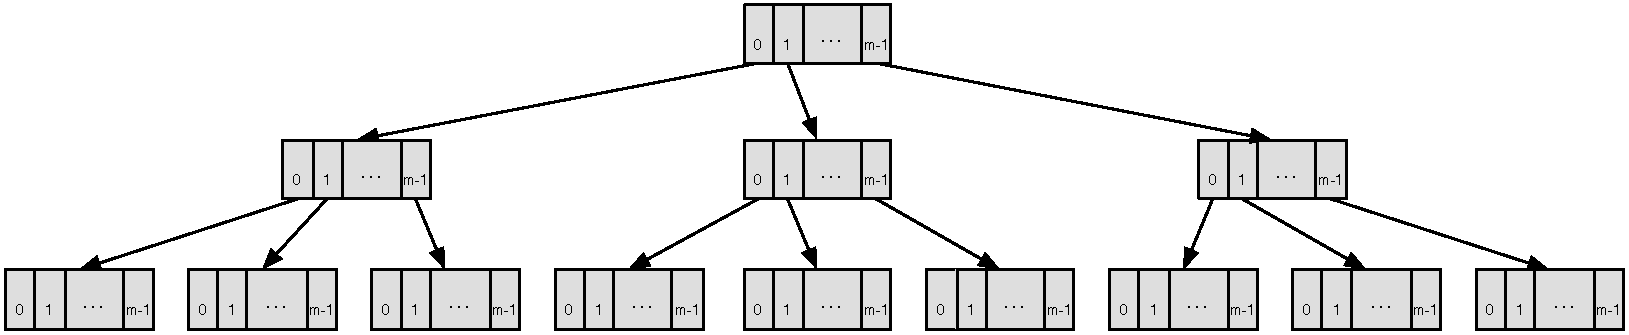
\includegraphics[width=\textwidth]{Figures/Radix_Balanced}
  \label{badix_balanced}
  \caption{Radix Balanced Tree Structure}
\end{figure}



%-----------------------------------
%	SUBSECTION - Operations
%-----------------------------------
\subsection{Operations}
% List core operations
% Hint of displays and transient states

%-----------------------------------
%	SUBSUBSECTION - Apply
%-----------------------------------

\subsubsection{Apply}
% used in head and last



%-----------------------------------
%	SUBSUBSECTION - Updated
%-----------------------------------

\subsubsection{Updated}
% base implementation needs to update the whole branch

% with transient states, local updates can be amortised

%-----------------------------------
%	SUBSUBSECTION - Additions
%-----------------------------------

\subsubsection{Additions}

\paragraph{Append and Prepend}
% base implementation needs to update the whole branch
% with transient states, consecutive appends are amortised

\paragraph{Concatenation and Insert}


%-----------------------------------
%	SUBSUBSECTION - Splits
%-----------------------------------

\subsubsection{Splits}
% used in tail, init, take, takeRight, drop, dropRight


%----------------------------------------------------------------------------------------
%	SECTION - Parallel Vectors
%----------------------------------------------------------------------------------------

\section{Parallel Vectors}

%-----------------------------------
%	SUBSUBSECTION - Splitter
%-----------------------------------

\subsection{Splitter Iterator}


%-----------------------------------
%	SUBSUBSECTION - Combiner
%-----------------------------------

\subsection{Combiner Builder}



%----------------------------------------------------------------------------------------
%	SECTION - Relaxed Radix Balanced Vectors
%----------------------------------------------------------------------------------------

\section{Relaxed Radix Balanced Vectors}

%-----------------------------------
%	SUBSECTION - Tree structure
%-----------------------------------

\subsection{Tree structure}
% describe tree: balancing, filling, block sizes

\begin{figure}[h!]
  \centering
  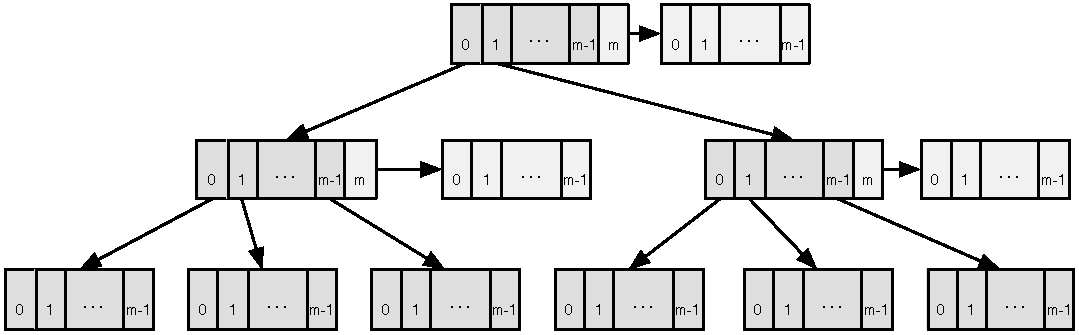
\includegraphics[width=\textwidth]{Figures/Relaxed_Radix_balanced}
  \label{Relaxed_Radix_balanced}
  \caption{Radix Balanced Tree}
\end{figure}

%-----------------------------------
%	SUBSECTION - Operations
%-----------------------------------
\subsection{Operations}
% List core operations
% Hint of displays and transient states

%-----------------------------------
%	SUBSUBSECTION - Apply
%-----------------------------------

\subsubsection{Apply (get element at index)}
% used in head and last


%-----------------------------------
%	SUBSUBSECTION - Updated
%-----------------------------------

\subsubsection{Updated}
% base implementation needs to update the whole branch

% with transient states, local updates can be amortised

%-----------------------------------
%	SUBSUBSECTION - Additions
%-----------------------------------

\subsubsection{Additions}

\paragraph{Append and Prepend}
% base implementation needs to update the whole branch
% with transient states, consecutive appends are amortised

\paragraph{Insert}


\paragraph{Concatenation}

\begin{figure}[h!]
  \centering
  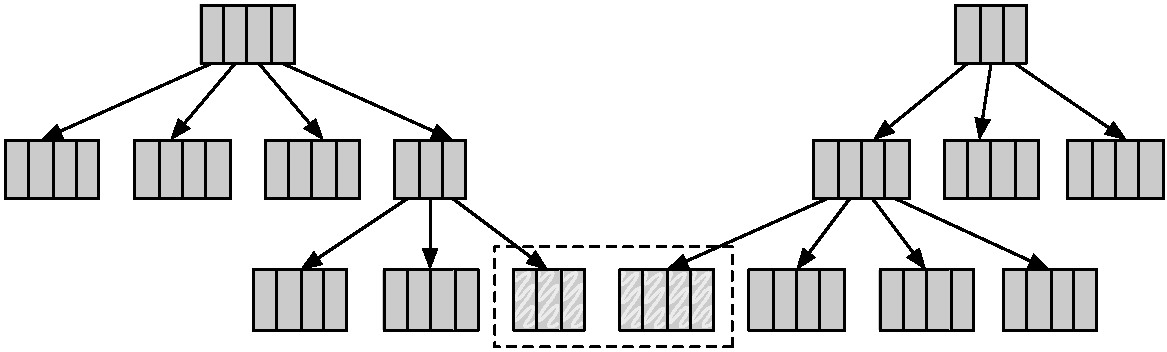
\includegraphics[width=\textwidth]{Figures/Concat0.pdf}
  \label{Concat0Benchmarks}
  \caption{Concatenation example with blocks of size 4: Rebalancing level 0}
\end{figure}

\begin{figure}[h!]
  \centering
  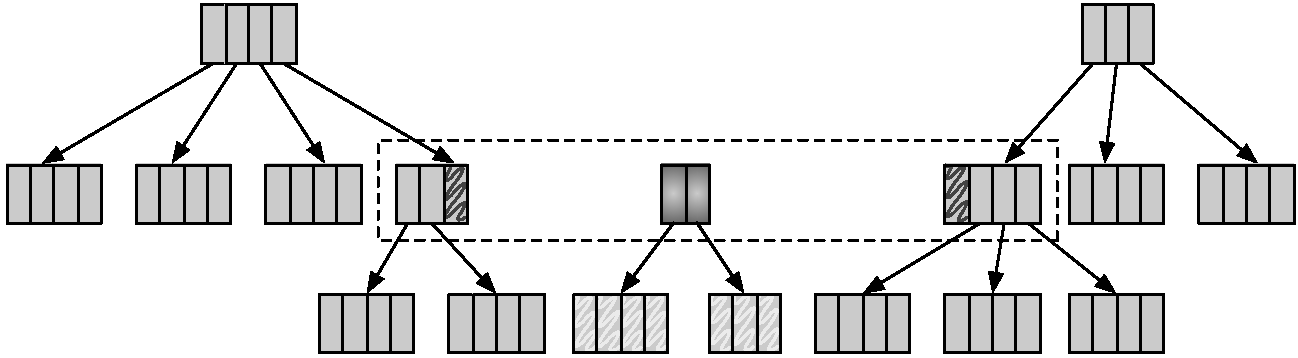
\includegraphics[width=\textwidth]{Figures/Concat1.pdf}
  \label{Concat1Benchmarks}
  \caption{Concatenation example with blocks of size 4: Rebalancing level 1}
\end{figure}

\begin{figure}[h!]
  \centering
  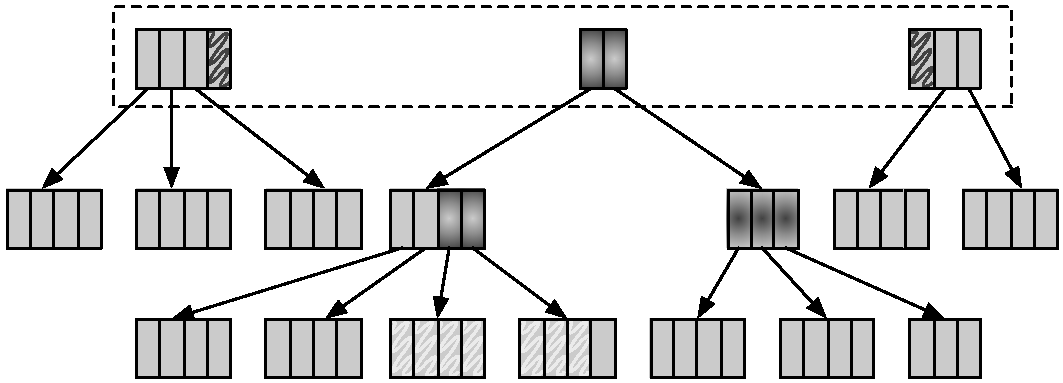
\includegraphics[width=\textwidth]{Figures/Concat2.pdf}
  \label{Concat2Benchmarks}
  \caption{Concatenation example with blocks of size 4: Rebalancing level 2}
\end{figure}

\begin{figure}[h!]
  \centering
  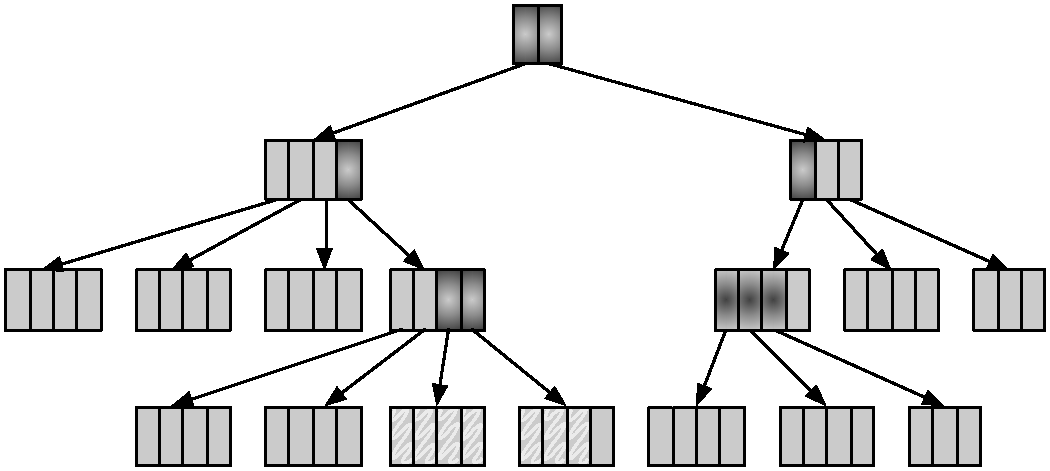
\includegraphics[width=\textwidth]{Figures/Concat3.pdf}
  \label{Concat3Benchmarks}
  \caption{Concatenation example with blocks of size 4: Rebalancing level 3}
\end{figure}

%-----------------------------------
%	SUBSUBSECTION - Splits
%-----------------------------------

\subsubsection{Splits}
% used in tail, init, take, takeRight, drop, dropRight



